%%%%%%%%%%%%%%%%%%%%%%%%%%%%%%%%%%%%%%%%%%%%%%%%%%
% 実行例(t=0) (第6章で使う)
%%%%%%%%%%%%%%%%%%%%%%%%%%%%%%%%%%%%%%%%%%%%%%%%%%

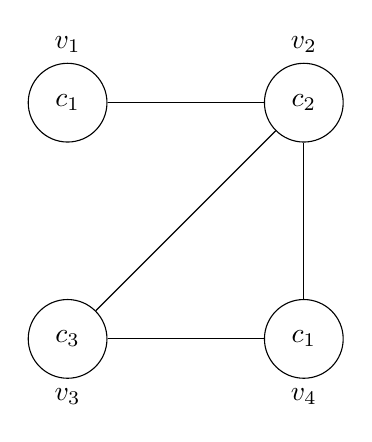
\begin{tikzpicture}[x=1.5cm, y=1.5cm]

  % 設定
  \tikzset{node/.style={circle,draw=black,minimum size=1cm}}
 

 
  % 補助線
  % \draw [help lines,blue] (0,0) grid (20,6);
 
  % node %
  \node[node, label=above:$v_1$] at (-1,1) (node1) {$c_1$};
  \node[node, label=above:$v_2$] at (1,1) (node2) {$c_2$};
  \node[node, label=below:$v_3$] at (-1,-1) (node3) {$c_3$};
  \node[node, label=below:$v_4$] at (1,-1) (node4) {$c_1$};
 
  \foreach \u / \v in {node1/node2, node2/node3, node2/node4, node3/node4}
  \draw (\u) -- (\v);
 \end{tikzpicture}
 
 %%%%%%%%%%%%%%%%%%%%%%%%%%%%%%%%%%%%%%%%%%%%%%%%%%%%%%%%%%
 %%% Local Variables:
 %%% mode: japanese-latex
 %%% TeX-master: paper.tex
 %%% End:
 